\item O disco está originalmente girando a $\omega_{0}=\SI{8}{\radian/\second}$. Se ele é submetido a uma aceleração angular constante $\alpha=\SI{6}{\radian/\second^{2}}$, determine a intensidade da velocidade e das componentes $n$ e $t$ da aceleração do ponto $B$ logo após o disco sofrer 2 revoluções.

\import{../answers/}{answer-3}

\vspace{-2cm}
\begin{flushright}
	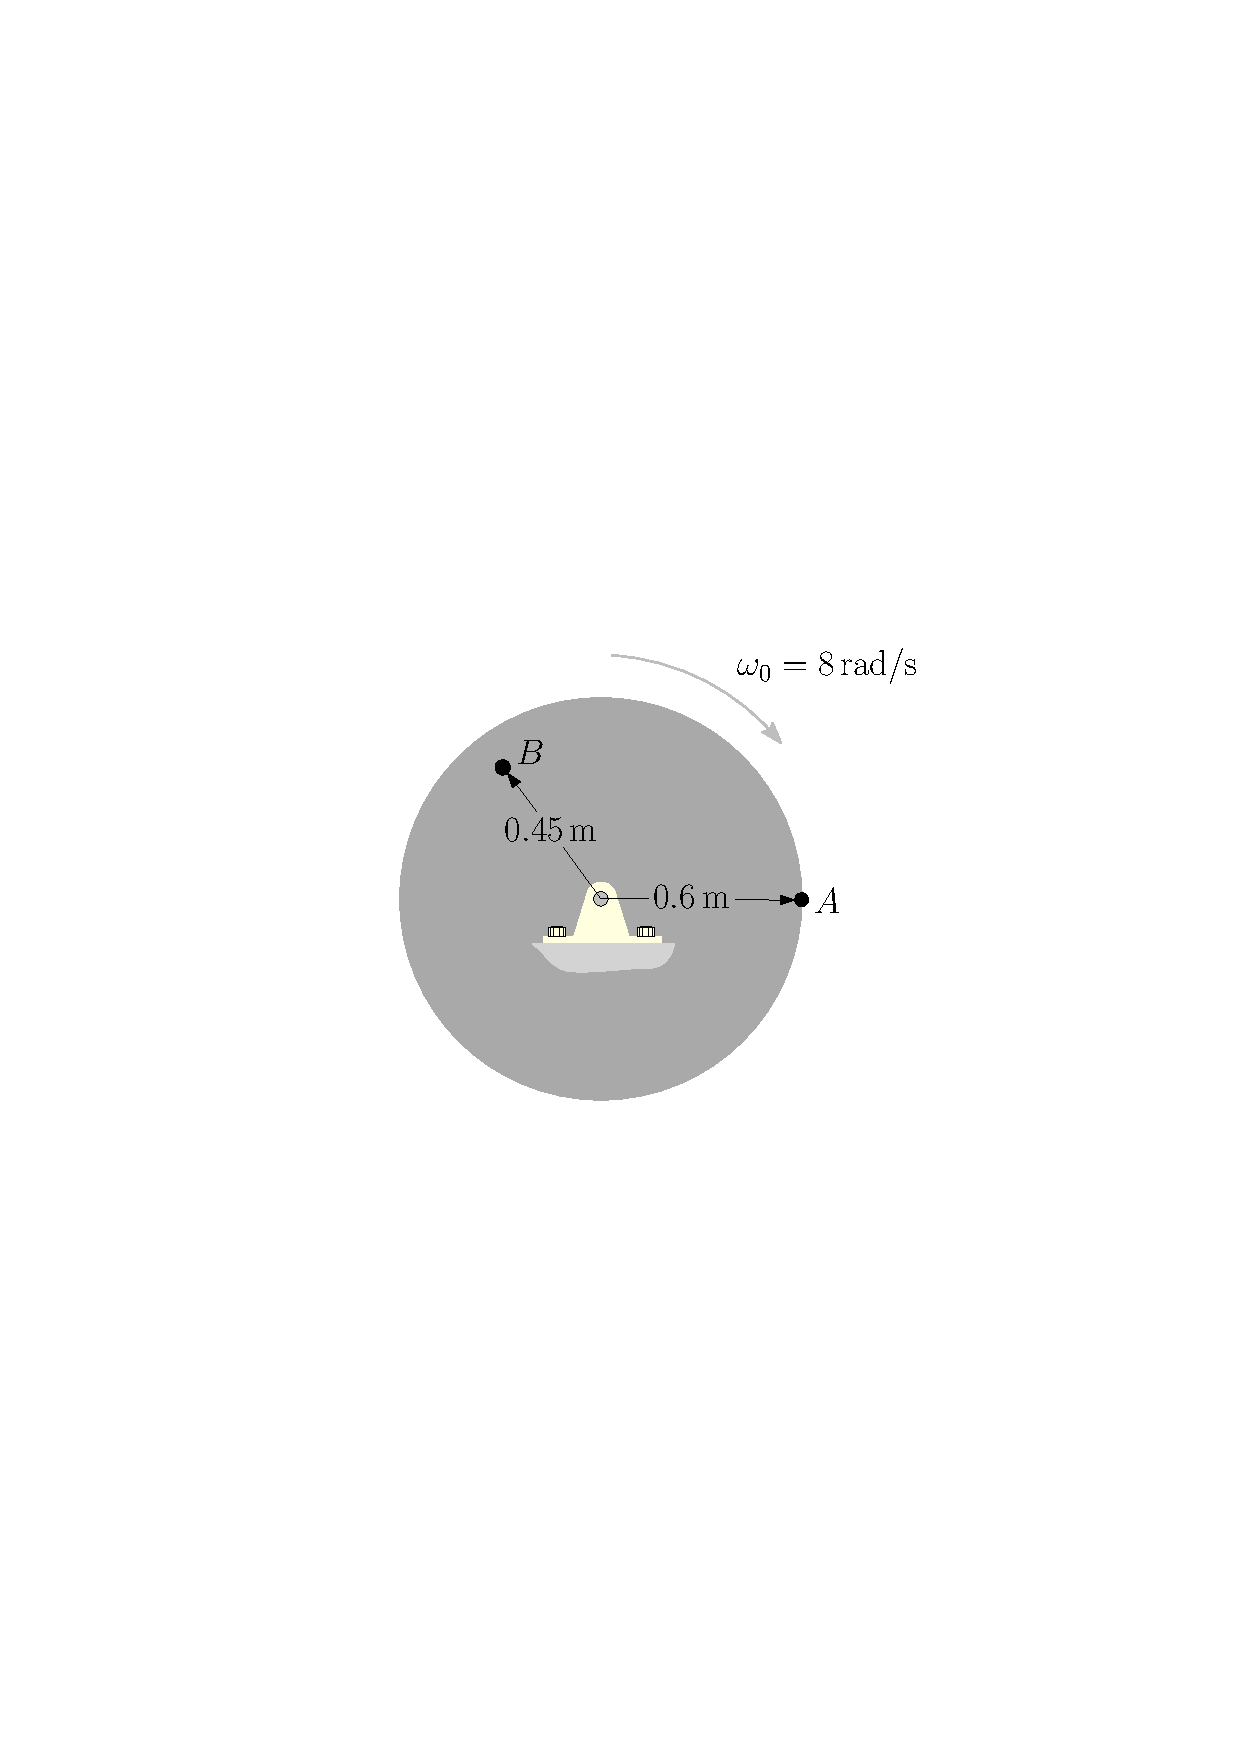
\includegraphics[scale=.75]{images/draw_8}
\end{flushright}